\documentclass[12pt]{article}

\usepackage[utf8]{inputenc}
\usepackage{setspace}
\usepackage{geometry}
\usepackage{graphicx}
\usepackage{caption}
\usepackage{indentfirst}
\usepackage{anyfontsize}
\usepackage{textcomp}
\usepackage{amsmath}
\usepackage{float}
\usepackage{changepage}
\usepackage [english]{babel}
\usepackage [autostyle, english = american]{csquotes}
\usepackage{tabto}
\usepackage{verbatim}
\usepackage{wrapfig}
\usepackage{caption}
\usepackage{subcaption}
\usepackage{stackengine}
\usepackage{scrextend}
\usepackage{booktabs}
\usepackage[table,xcdraw]{xcolor}
\usepackage{cite}
\usepackage{nicefrac}
\usepackage[numbers, comma, super, square]{natbib}

\graphicspath{}
\MakeOuterQuote{"}

\title{Mapping Stable Manifolds}
\author{Geneva Porter and Lyndsay Walker}
\date{17 December 2018}

\begin{comment}

\begin{figure}[H]
\centering{\includegraphics[width=10cm]{FILENAME.eps}}
\caption*{\textbf{CAPTION}}
\end{figure}

$\begin{bmatrix}
11      & 12  \\
21      & 22  \\
\end{bmatrix}$

\end{comment}

\begin{document}
	
\begin{titlepage}
\maketitle
\thispagestyle{empty}


\begin{center}
	
\large \it San Diego State University 
	
Professor A Palacios, Math 538

\end{center}
\end{titlepage}

\section{Introduction}

	Historically, approximating manifolds has been a challenge in discrete systems analysis due to the absence of analytical solutions. Stable manifolds in particular are often elusive, especially when inverse iterations diverge quickly or the inverse cannot be computed explicitly. Krauskopof \textit{et. al} (1998) and England \textit{et. al} (2004) each developed a method of computing one-dimensional stable manifolds that can be applied to two-dimensional discrete systems. We will summarize the implementation of these two methods, highlighting the costs and benefits of both.
	
	Krauskopof's algorithm assumes that the inverse map is known. This method uses an inverse map to plot successive points in the desired manifold. Because the inverse is known, Krauskopof's method can be used to plot either the unstable manifold using the given function or the stable manifold using the inverse function. Alternatively, England's algorithm assumes the inverse map is not known, but still applies to finding either the stable manifold or the unstable manifold. This method uses educated guesses for successive points and tests those guesses several times for each step. We will summarize both these methods in relation to finding the stable manifold.
	
	While their algorithms differ, two elements of these methods are identical. Both methods require a "seed" of iteration on the stable manifold. This seed is found by choosing a point near the saddle point $x_0$ in the direction indicated by the eigenvector corresponding to the non-dominant eigenvalue. In addition, both methods utilize a "search circle," which is established to estimate the distance between points on the stable manifold. A value $\Delta_k$ is chosen as this estimate and used as the radius of the search circle centered at $p_k$, the starting point for each loop of the algorithm. Both methods also include similar processes for determining the validity of each approximation. The next sections summarize these methods in more detail. 

\section{Stable Manifold by Using the Inverse}

	Plotting the stable manifold of a discrete map when the inverse is known is generally simpler than plotting without a known inverse. We will examine an algorithm for plotting the stable manifold using an inverse map, as given by Krauskopof. Note that while the algorithm is designed to plot the \textit{unstable} manifold, simply substituting the inverse function will yield a map of the \textit{stable} manifold. To avoid confusion, consider a map $f(x,y)$ is given, and we wish to approximate the stable manifold. The inverse of $f$ will be defined as $f^{-1}(x,y)=g(x,y)$. To find the stable manifold of $f$, we will calculate the unstable manifold of $g$. The notation $g$ and $g^{-1}$ will be used when summarizing this algorithm procedure. 
	
	To begin plotting the unstable manifold of $g$, locate the saddle point and create a linear approximation in the direction of the unstable manifold. This linear approximation forms a piecewise mesh. Before summarizing this algorithm, we will assume there is already a series of points $M=\{p_0,p_1,...,p_{k-1},p_k\}$ built up on the manifold. Beginning at $p_k$, establish the search circle, $C(p_k,\Delta_k)$. Next, locate the pre-image of $p_k$ by evaluating $g^{-1}(x,y)$. If the map is not orientation-preserving, then the second iteration $g^{-1}(g^{-1}(x,y))$ must be used. Using the mesh approximation line, move linearly through the mesh until a segment $L$ is found whose image under $g$ intersects the search circle. Then, choose a point $q$ on the line segment that maps near the intersection point, within some tolerance $\varepsilon$ from the edge of the search circle. Figure \ref{figure:winverse} shows a visualization for this algorithm, taken from Krauskopf's article. Note that $W^u_{pl}(x_0)$ denotes the unstable manifold approximation of $g$ about the saddle point $x_0$ that has already been calculated.
	
	\begin{figure}[H]
	\centering{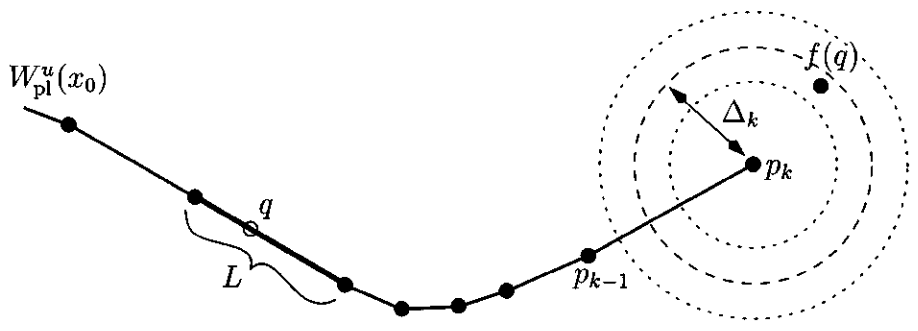
\includegraphics[width=10cm]{winverse.png}}
	\caption{Process for finding $p_{k+1}$ using the inverse map}
	\label{figure:winverse}
    \end{figure}
	
	Once $q$ has been found, check to see of the point $p_{k+1}=g(q)$ is an adequate addition to the manifold by approximating the angle, $\alpha_k$, made by $p_{k-1}$, $p_k$, and $p_{k+1}$. This approximation is given by:
	
	\begin{equation}\label{alpha1}
	\alpha_k=\dfrac{||\bar{p}-p_{k-1}||}{||p_k-p_{k-1}||}\hspace{5mm} \textrm{with} \hspace{5mm} \bar{p}=p_k+\dfrac{p_k-p_{k+1}}{||p_k-p_{k-1}||}
	\end{equation}
	
	If $\alpha_k$ does not fall within a predefined tolerance, then perform the algorithm again and use $\frac{\Delta_k}{2}$ as the radius of the search circle. If $\alpha_k$ is acceptable, then $p_{k+1}$ is accepted and recorded for for plotting later. The mesh can now be redefined using a linear approximation in the direction of the non-dominant eigenvalue at $p_{k+1}$. Repeat this process until the manifold is adequately built.

\section{Stable Manifold Without Using the Inverse}

	This algorithm grows a branch of the stable manifold based on previously computed points in the manifold via a search circle. This search circle algorithm works differently than the one presented in the above section in that it does not use $f^{-1}$ for finding the next point in the manifold. Instead, it finds the next point in the manifold, close to the most recently computed point, which maps to a piece of the manifold already computed.
	
	The initial point in the stable manifold is the saddle node, denoted $p_0$. The next point is a $\delta>0$ distance away from $p_0$ in the direction of the stable eigenvector. The distance between two points, $p_i, p_{i+1}$, is adjusted according to the angles between three consecutive line segments.
	
	Consider a branch of a stable manifold which consists of an ordered set of points at varying distances, $M = \{p_0, p_1, \dots, p_{k-1}, p_k\}$. Using the last point, $p_k$, we attempt to find $p_{k+1}$ at some $\Delta_k$ distance away, creating $C(p_k, \Delta_k)$. This circle is constructed to intersect the manifold in two locations. One intersection is on the line segment $[p_{k-1},p_k]$, which is already known and not of interest. The other intersection is where $p_{k+1}$ is located, this is what we are interested in finding.
	
	The image of the circle, $f(C(p_k, \Delta_k))$, will map to a previously computed portion of the stable manifold and will intersect at two locations. One of those locations corresponds to the known intersection of $C(p_k,\Delta_k)$, the other corresponds to $f(p_{k+1})$. The latter is the intersection we wish to find. This crossing will occur at a known line segment between two consecutive points in the manifold. The line segment will be assumed to be the one which contained $f(p_k)$, and we will call it $[p_{i-1}, p_i]$.
	
	The candidate points for $p_{k+1}$ are selected from an arc of the $C(p_k,\Delta_k)$ with angle $\alpha_k$, $C_{\alpha_k}(p_k,\Delta_k)$.  The beginning search point on the arc, $p_{start}$, and terminal, $p_{end}$, should have images on opposite sides of $[p_{i-1}, p_i]$. This is done by checking the projection of the points onto the normal of the line. If the images are on the same side, then $\alpha_k$ is increased. This ensures that $f(C_{\alpha_k}(p_k, \Delta_k))$ will intersect the line segment.
	
	To ensure that we are getting an acceptable resolution of the manifold, we monitor $\alpha_k$, which is the angle between $p_{k-1}, p_k,$ and $p_{k+1}$. An approximate $\alpha_k$ is given by:
	
	$$\alpha_k = 2\sin^-1\left( \frac {|| \bar{p} -p_{k-1}||}{2||p_k-p_{k-1}}\right) \approx \left( \frac {|| \bar{p} -p_{k-1}||}{2||p_k-p_{k-1}}\right)\text{,} $$
	
	$$\text{where \hspace{5mm}}\bar{p} = p_k+\frac{||p_k -P_{k-1}||}{||p_k-p_{k+1}||} (p_k-p_{k+1})$$
	
	The angle is now bisected and the point on the arc corresponding to the bisection is $p_{try}$. Again, we look at the image, $f(p_{try})$, and check how far away from the line segment it is. Once it is less than some $\epsilon_B$ distance away, we accept this point as the candidate point for $p_{k+1}$. Figure \ref{figure:ninverse} gives a pictorial representation of this process.\\
	\begin{figure}[H]
	\centering{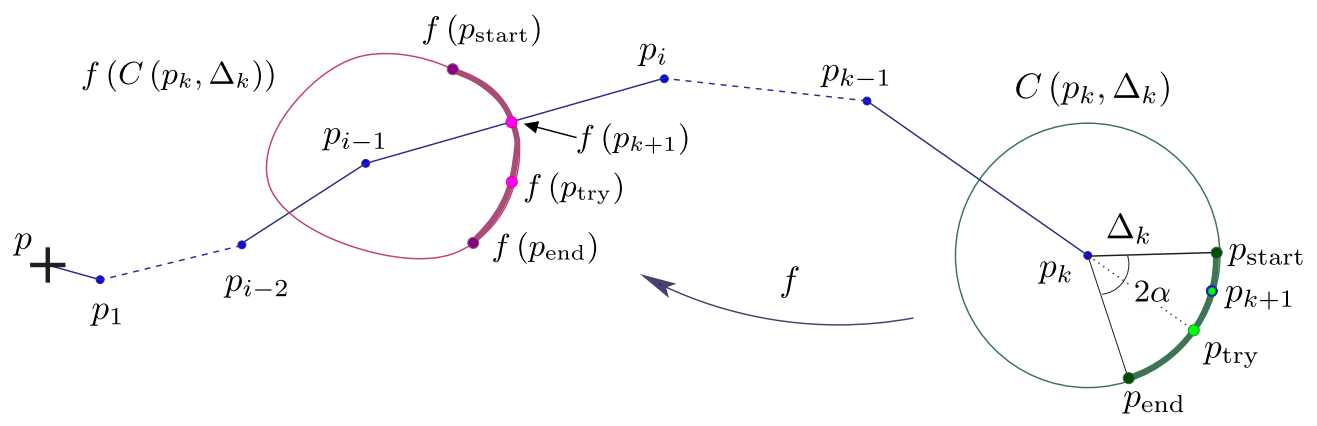
\includegraphics[width=14cm]{ninverse.png}}
	\caption{Process for finding $p_{k+1}$ without using the inverse map}
	\label{figure:ninverse}
    \end{figure}
	The last step is to check that $f(p_{try})$ is on the line segment previously assumed. To do this, we check that the projection, $\tau$ of the point, $f(p_{try})$ onto the line segment. If $\tau<0$ we move to the previous line segment and run the algorithm again. If $\tau>1$ we move to the next line segment and run the algorithm again. Otherwise, $0\leq \tau \leq 1$, we are on the line segment and $p_{try}$ is accepted as $p_{k+1}$ and is added to the manifold. 

\section{Results}

    Both methods can be utilized to find either the stable or the unstable manifolds. A comparison of implementations from method is given in figure \ref{figure:shear} below, using the shear map as a basis for evaluation. Both implementations plot both the stable and unstable manifolds, and appear to be a visual match. This indicates that the methods described above are both valid for mapping either manifold type. Although mapping stable manifolds when the inverse is known is generally less complicated, often the inverse cannot be found either analytically or approximated numerically, such as with Newton's Method. One example of a non-invertible map is the tent map, as the modulus function is not one-to-one and therefore does not have an inverse. England's method can be used to give an accurate picture of the desired manifold in instances like this.

	\begin{figure}[H]
	\centering{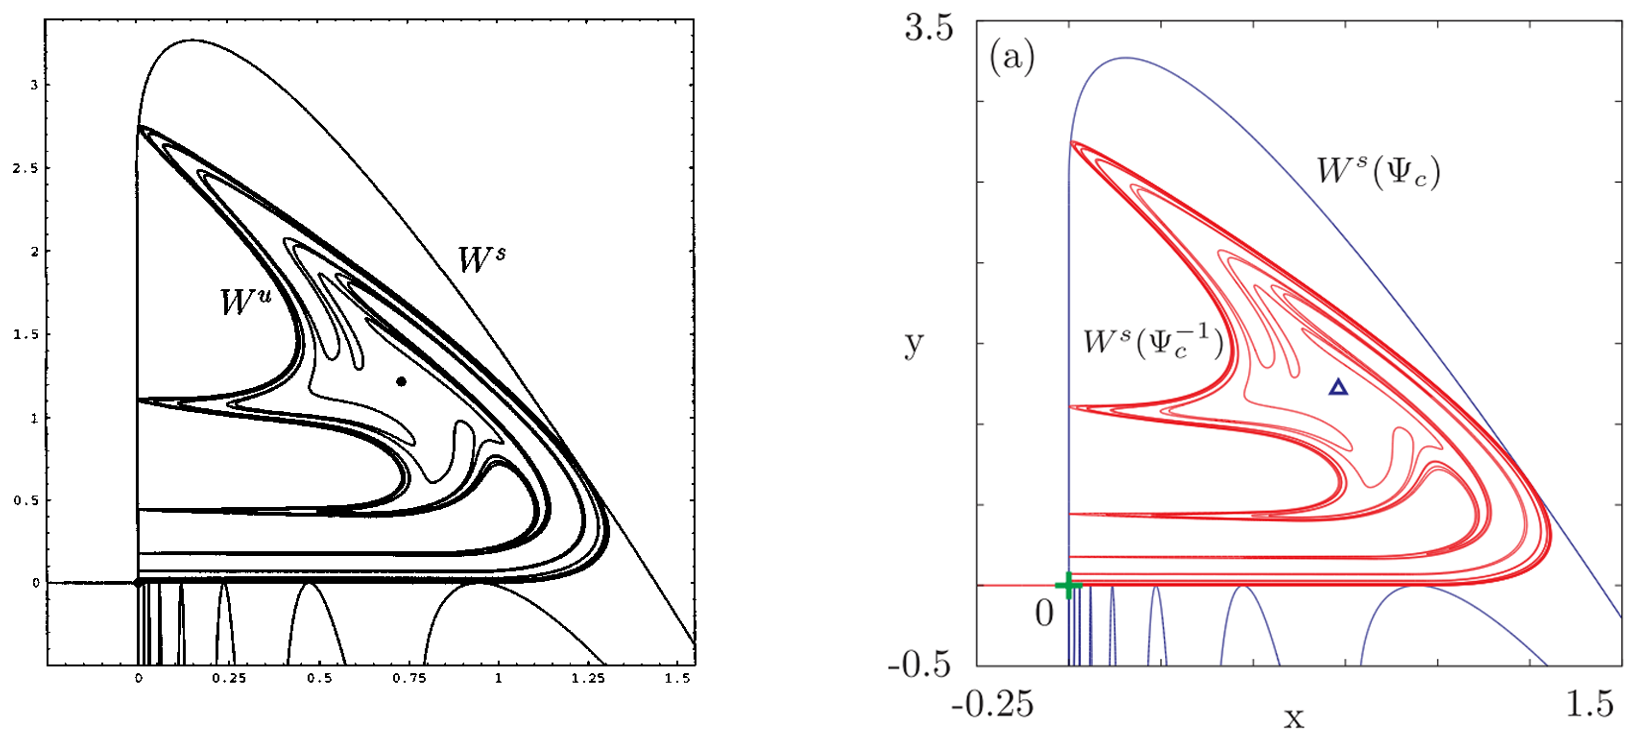
\includegraphics[width=14cm]{shear.png}}
	 \caption{\centering Shear map implementations using both methods. \\ \centering Left: Method with the inverse\cite{Krauskopf1998} \hspace{3mm} Right: Method without the inverse\cite{England2004}}
	\label{figure:shear}
    \end{figure}



\section{Conclusion}
The methods presented in this paper have been applied specifically to two-dimensional maps, which create one-dimensional manifolds. The next logical step would be to extend the results to three- and four-dimensional maps. The values for $p_0$ and $p_1$ would be found in the same manner. However, greater attention will need to be given to building the two-dimensional visualization. One possible solution is to create the manifold in a similar manner described above, however each point must be extended into a line orthogonal to the points found to be in the manifold. The endpoints of the orthogonal lines should be used to create another set of points, as previously described. It will be interesting to see where the research and applications for these methods will lead.
 


\subsection*{References}
\begingroup
\renewcommand{\section}[2]{}%
\nocite{*}
\bibliographystyle{acm}
\bibliography{538Final}
\endgroup




\end{document}


